\section{Unauthenticated user}
\subsection{Signing up}
If you wish to sign up to \textit{EmporioLambda}, access any page of the website. In the header section of the page you'll see a button with the text 'Register / Sign in'. Clicking it will redirect you to the login page.

\begin{figure}[H]
\centering

\includegraphics[scale=0.6]{res/Immagini/RegisterSigninButton}
\caption{Registration and sign in button}
\end{figure}

To proceed with the sign up procedure you will then have to click the 'Sign up' text. In the following picture, it is highlighted in red.

\begin{figure}[H]
\centering
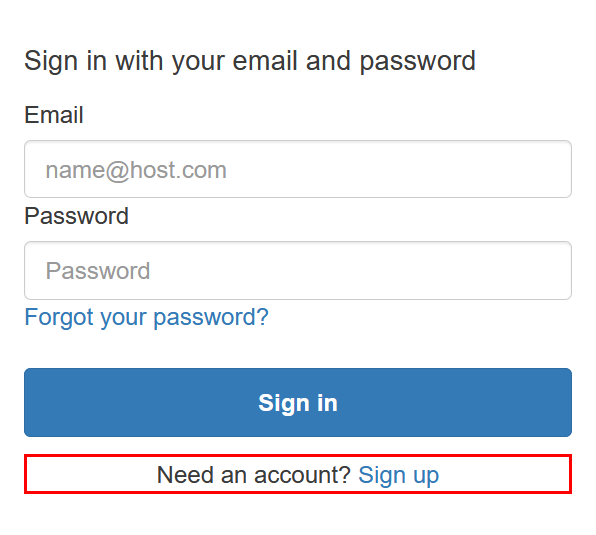
\includegraphics[scale=0.6]{res/Immagini/RegisterSigninForm}
\caption{Login form}
\end{figure}

You will then find yourself on page with a form to insert your data. Every field is mandatory, and the system will not let you continue unless all the necessary data is present. 

The password field must contain a lower case letter, an upper case letter, a special character, a number and must be at least 8 characters long.

\begin{figure}[H]
\centering
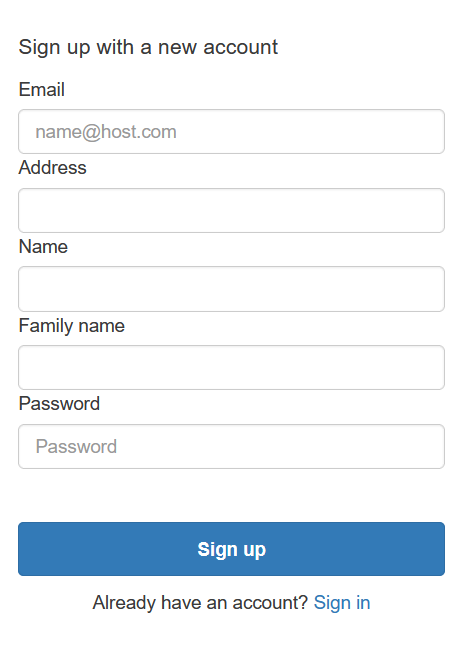
\includegraphics[scale=0.6]{res/Immagini/RegisterForm}
\caption{Sign up form}
\end{figure}

After compiling every field and clicking on the 'Sign up' button, you will see a page asking for a confirmation code. You will receive this code by email, on the address you specified in the last step. After inserting the code and clicking on the 'Confirm Account' button, you will have successfully completed the sign up procedure. You will therefore be redirected to the homepage, already signed in.

If, after waiting a few minutes, you still haven't received your confirmation code, you can try clicking on the 'Resend it' text to send it again.

\begin{figure}[H]
\centering
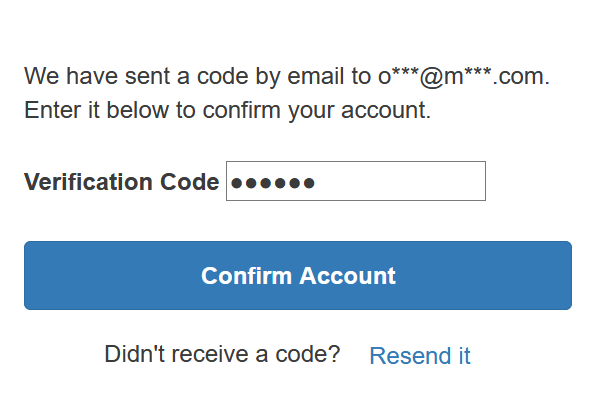
\includegraphics[scale=0.6]{res/Immagini/RegisterCode}
\caption{Confirmation code form}
\end{figure}

\subsubsection{Sign up error}
If any error happen during the registration procedure, you will be redirected to the previous section with an error message describing what the problem is. If the message isn't self explanatory, please refer to section 7-Bug reporting.

\begin{figure}[H]
\centering
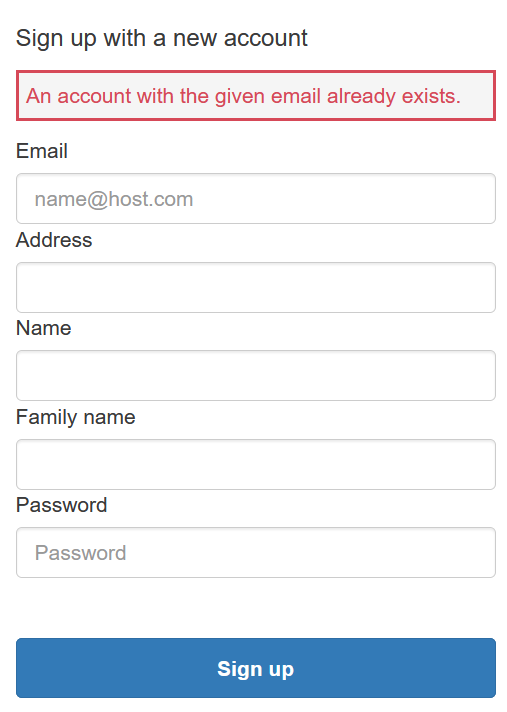
\includegraphics[scale=0.6]{res/Immagini/RegisterError}
\caption{Sign up error example: the email address is already in use}
\end{figure}

\subsection{Signing in}
In order to sign in to \textit{EmporioLambda}, an account is needed. If an account hasn't yet been created, refer to section 1-Signing up.

To sign in, access any page of the website. In the header section of the page you'll see a button with the text 'Register / Sign in'. Clicking it will redirect you to the login page.

\begin{figure}[H]
\centering

\includegraphics[scale=0.6]{res/Immagini/RegisterSigninButton}
\caption{Registration and sign in button}
\end{figure}

To proceed with the sign in procedure you will then have to insert your data in the sign in form. After compiling the form, click on the 'Sign in' button. If the email and password were correct, you will be redirected to the homepage of the website, successfully logged in.

\begin{figure}[H]
\centering
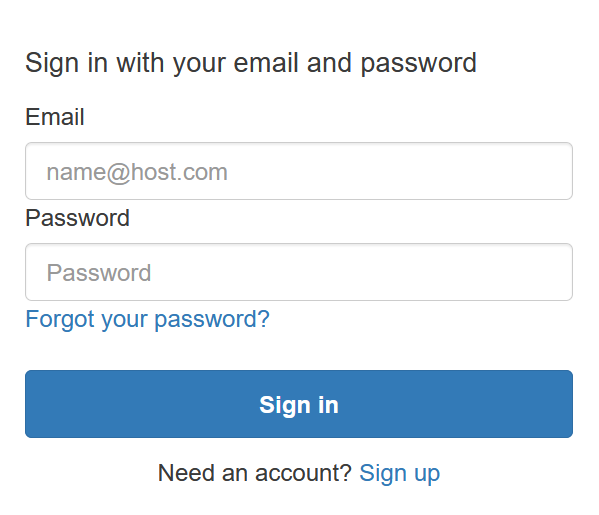
\includegraphics[scale=0.6]{res/Immagini/SigninForm}
\caption{Sign in form}
\end{figure}

\subsubsection{Forgotten password}
If you forgot your login password, click on the 'Forgot your password?' text. You will have to then insert your account's email and click on the 'Reset my password' button in order to continue.

\begin{figure}[H]
\centering
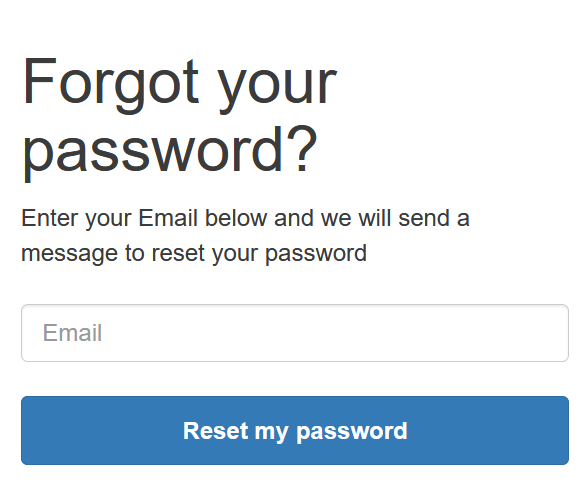
\includegraphics[scale=0.6]{res/Immagini/ResetPassword}
\caption{Forgot your password page}
\end{figure}

You will then have to fill a form with your new password. You will also receive a confirmation code by email, on the address you specified in the last step. This code will also have to be inserted in the form in order to reset your password.

Once the form is filled, click on the 'Change Password' button to reset your password. You will then be redirected to the login form, with your password updated.

\begin{figure}[H]
\centering
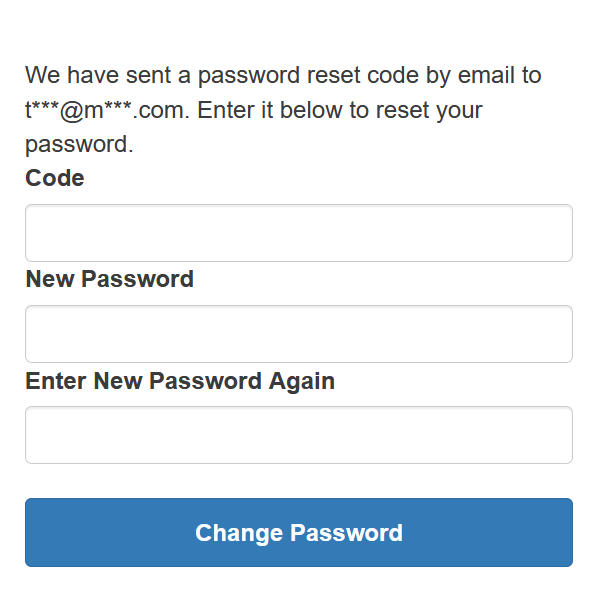
\includegraphics[scale=0.6]{res/Immagini/ResetPasswordForm}
\caption{Forgot your password page}
\end{figure}

\subsubsection{Sign in error}
If any error happen during the login procedure, you will be redirected to the previous section with an error message describing what the problem is. If the message isn't self explanatory, please refer to section 7-Bug reporting.

\begin{figure}[H]
\centering
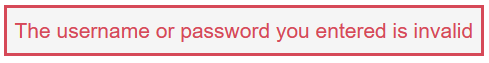
\includegraphics[scale=0.6]{res/Immagini/SigninError}
\caption{Sign in error example: the email or password entered was invalid}
\end{figure}

\subsection{Signing out}
In order to sign out of \textit{EmporioLambda}, you must first be logged in. You will then see, in any page of the website, a 'Sign out' button. Press this button to be logged off the website.

\begin{figure}[H]
\centering
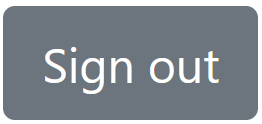
\includegraphics[scale=0.6]{res/Immagini/SignoutButton}
\caption{Sign out button}
\end{figure}
